\documentclass{article}

\usepackage{geometry}
\usepackage{amsmath}
\usepackage{graphicx, eso-pic}
\usepackage{listings}
\usepackage{hyperref}
\usepackage{multicol}
\usepackage{fancyhdr}
\pagestyle{fancy}
\fancyhf{}
\hypersetup{ colorlinks=true, linkcolor=black, filecolor=magenta, urlcolor=cyan}
\geometry{ a4paper, total={170mm,257mm}, top=10mm, right=20mm, bottom=20mm, left=20mm}
\setlength{\parindent}{0pt}
\setlength{\parskip}{0.3em}
\renewcommand{\headrulewidth}{0pt}

\rfoot{\thepage}
\fancyhf{} % sets both header and footer to nothing
\renewcommand{\headrulewidth}{0pt}
\lfoot{\textbf{OHL Labpro 2024}}
\pagenumbering{gobble}

\fancyfoot[CE,CO]{\thepage}
\lstset{
    basicstyle=\ttfamily\small,
    columns=fixed,
    extendedchars=true,
    breaklines=true,
    tabsize=2,
    prebreak=\raisebox{0ex}[0ex][0ex]{\ensuremath{\hookleftarrow}},
    frame=none,
    showtabs=false,
    showspaces=false,
    showstringspaces=false,
    prebreak={},
    keywordstyle=\color[rgb]{0.627,0.126,0.941},
    commentstyle=\color[rgb]{0.133,0.545,0.133},
    stringstyle=\color[rgb]{01,0,0},
    captionpos=t,
    escapeinside={(\%}{\%)}
}

\begin{document}

\begin{center}
    \section*{Bantu Purry si Platypus Mewing Menemukan String Sigma!} % ganti judul soal

    \begin{tabular}{ | c c | }
        \hline
        Batas Waktu  & 3s \\    % jangan lupa ganti time limit
        Batas Memori & 256MB \\  % jangan lupa ganti memory limit
        \hline
    \end{tabular}
\end{center}

\subsection*{Deskripsi}

Suatu hari, Purry si Platypus yang punya rizz tingkat tinggi lagi mewing di pantai dan tiba-tiba menemukan teka-teki yang bikin otaknya kerja keras banget!

Jadi, bantuin Purry menyelesaikan teka-teki ini supaya dia bisa kembali menikmati harinya dengan tenang tanpa harus kena fanum tax! Kalau berhasil, Purry bakal sangat berterima kasih dengan gyatt yang besar!

Nah, ceritanya ada sebuah string $s$ yang harus dienkripsi. Caranya, semua 26 huruf kecil alfabet diatur dalam lingkaran dengan urutan tertentu. Terus, setiap huruf dalam $s$ diganti dengan huruf yang mengikutinya dalam urutan searah jarum jam. Begitu caranya string $x$ diperoleh.

Nah, lo dikasih string $x$. Tugas lo adalah bantuin Purry si Platypus nemuin string $s$ yang bisa jadi prototipe dari string $x$ dan merupakan string terkecil secara leksikografis.

\begin{itemize}
\item Sebuah string $a$ lebih kecil secara leksikografis daripada string $b$ dengan panjang yang sama jika dan hanya jika:
\begin{itemize}
\item Pada posisi pertama di mana $a$ dan $b$ berbeda, string $a$ punya huruf yang muncul lebih awal dalam alfabet daripada huruf yang sesuai dalam $b$.
\end{itemize}
\end{itemize}

\subsection*{Format Masukan}

Baris pertama dari input berisi sebuah bilangan bulat $t$ $(1 \leq t \leq 3 \cdot 10^4)$, jumlah kasus uji.

Baris pertama dari setiap kasus uji berisi satu bilangan bulat $n$ $(1 \leq n \leq 10^5)$, panjang string $x$.

Baris berikutnya berisi string $x$ dengan panjang $n$, yang terdiri dari huruf kecil alfabet.

Dijamin bahwa jumlah $n$ dari semua kasus uji tidak melebihi $2 \cdot 10^5$.



\subsection*{Format Keluaran}

Untuk setiap kasus uji, keluarkan satu baris yang berisi string $s$ yang paling kecil secara leksikografis yang bisa menjadi prototipe dari $x$.

\\

\begin{multicols}{2}
\subsection*{Contoh Masukan}
\begin{lstlisting}
4
1
a
2
ba
15
purrysiplatypus
26
abcdefghijklmnopqrstuvwxyz

\end{lstlisting}
\columnbreak
\subsection*{Contoh Keluaran}
\begin{lstlisting}
b
ac
abccdefaghidabe
bcdefghijklmnopqrstuvwxyza
\end{lstlisting}
\end{multicols}

\subsection*{Penjelasan}
Dalam kasus uji pertama, kita tidak bisa menggunakan string "a", karena huruf a akan bertransisi ke dirinya sendiri. Secara leksikografis, string kedua "b" cocok sebagai jawaban.

Dalam kasus uji kedua, string "aa" tidak cocok, karena a akan bertransisi ke dirinya sendiri. "ab" tidak cocok, karena lingkaran akan ditutup dengan 2 huruf, tetapi harus mengandung semua 26 huruf. String berikutnya "ac" cocok.

\begin{minipage}{0.5\textwidth}
  Di samping ini, Anda dapat melihat skema untuk dua kasus uji pertama. Huruf-huruf yang tidak terlibat diabaikan, mereka bisa ditempatkan secara sembarang di celah-celah.
\end{minipage}
\begin{minipage}{0.5\textwidth}
  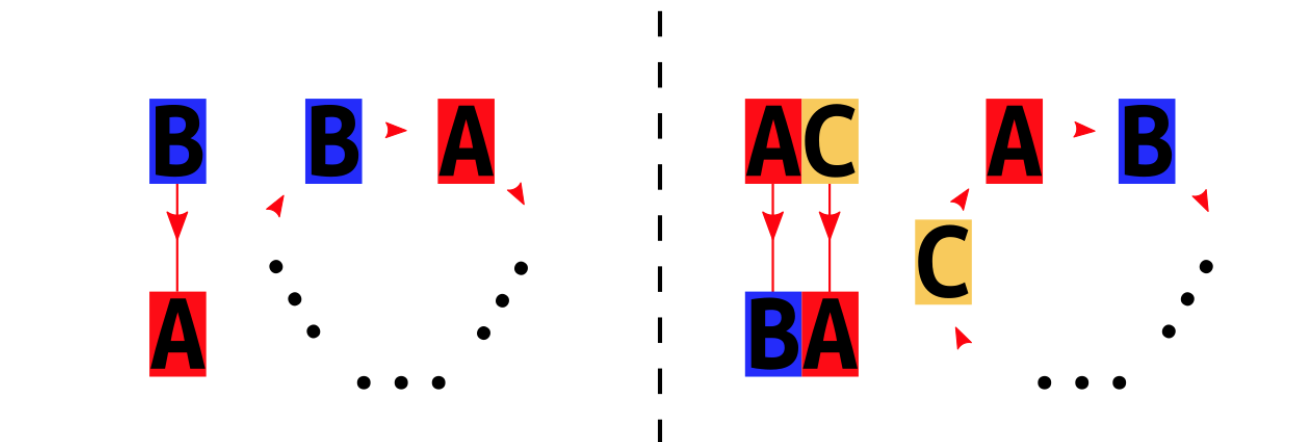
\includegraphics[width=\linewidth]{gambar_penjelasan.png}
\end{minipage}%


\end{document}